\documentclass[tikz,border=6pt]{standalone}
\usepackage[T1]{fontenc}
\usepackage{times}
\usepackage{amsmath,amssymb,bm}
\DeclareMathOperator*{\argmin}{arg\,min}
\usetikzlibrary{arrows.meta, positioning, fit, backgrounds, calc, decorations.pathreplacing}
\pgfdeclarelayer{deepbg}
\pgfsetlayers{deepbg,background,main}

% Colors
\definecolor{envcolor}{HTML}{D4E6F1}
\definecolor{envborder}{HTML}{2980B9}
\definecolor{nncolor}{HTML}{FAD7A0}
\definecolor{nnborder}{HTML}{E67E22}
\definecolor{mpccolor}{HTML}{A9DFBF}
\definecolor{mpcborder}{HTML}{27AE60}
\definecolor{criticcolor}{HTML}{D7BDE2}
\definecolor{criticborder}{HTML}{8E44AD}
\definecolor{actorbg}{HTML}{FEF9E7}
\definecolor{actorborder}{HTML}{D4AC0D}
\definecolor{agentbg}{HTML}{F8F9F9}
\definecolor{agentborder}{HTML}{ABB2B9}
\definecolor{sharecolor}{HTML}{E74C3C}
\definecolor{neuroncolor}{HTML}{5DADE2}

\begin{document}
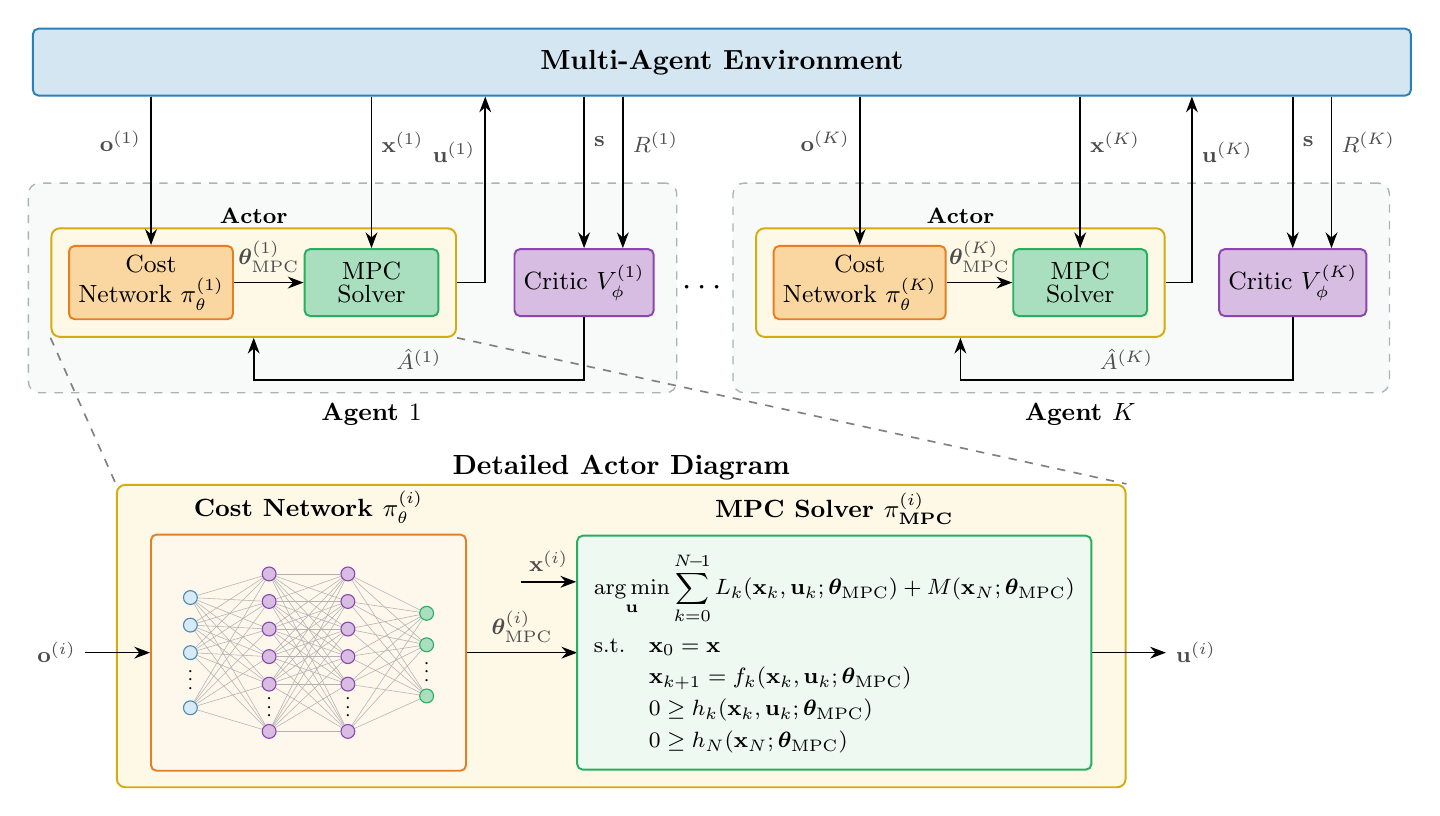
\begin{tikzpicture}[
    >=Stealth,
    block/.style={draw, rounded corners=2pt, minimum height=0.85cm,
        minimum width=1.7cm, align=center, font=\small, line width=0.7pt},
    env/.style={block, fill=envcolor, draw=envborder,
        minimum width=17.5cm, font=\normalsize\bfseries},
    nn/.style={block, fill=nncolor, draw=nnborder},
    mpc/.style={block, fill=mpccolor, draw=mpcborder},
    critic/.style={block, fill=criticcolor, draw=criticborder},
    actorbox/.style={draw=actorborder, rounded corners=3pt,
        fill=actorbg, inner sep=6pt, line width=0.7pt},
    agentbox/.style={draw=agentborder, rounded corners=4pt,
        fill=agentbg, inner xsep=8pt, inner ysep=16pt, line width=0.5pt, dashed},
    dl/.style={font=\footnotesize, text=black!70},
    arr/.style={->, line width=0.6pt},
    sharr/.style={<->, line width=0.7pt, dashed, color=sharecolor},
    neuron/.style={circle, draw=neuroncolor!80!black, fill=neuroncolor!25,
        minimum size=5pt, inner sep=0pt, line width=0.4pt},
    mpcdetail/.style={draw=mpcborder, rounded corners=2pt,
        fill=mpccolor!20, inner sep=6pt, line width=0.7pt,
        align=left, font=\footnotesize},
    nndetail/.style={draw=nnborder, rounded corners=2pt,
        fill=nncolor!20, inner sep=6pt, line width=0.7pt},
    detailbox/.style={draw=black!40, rounded corners=4pt,
        fill=white, inner sep=10pt, line width=0.6pt},
]

% ==========================================================
% ENVIRONMENT
% ==========================================================
\node[env] (env) at (1.25, 0) {Multi-Agent Environment};

% ==========================================================
% AGENT 1 — horizontal pipeline
% ==========================================================
\node[nn] (nn1) at (-6.0, -2.8) {\shortstack{Cost\\[-1pt] Network $\pi^{(1)}_\theta$}};
\node[mpc] (mpc1) at (-3.2, -2.8) {\shortstack{MPC\\[-1pt] Solver}};
\node[critic] (crit1) at (-0.5, -2.8) {\shortstack{Critic $V^{(1)}_\phi$}};

% Actor box
\begin{scope}[on background layer]
\node[actorbox, fit=(nn1)(mpc1),
    label={[font=\footnotesize\bfseries, yshift=-2pt]above:Actor}] (act1) {};
\end{scope}
% Agent box
\coordinate (ag1pad) at ([yshift=-0.4cm]crit1.south);
\begin{pgfonlayer}{deepbg}
\node[agentbox, fit=(act1)(crit1)(ag1pad)] (ag1) {};
\node[font=\small\bfseries, anchor=north] at (ag1.south -| mpc1) {Agent $1$};
\end{pgfonlayer}

% Internal arrow: NN -> MPC
\draw[arr] (nn1) -- node[dl, above] {$\bm{\theta}^{(1)}_{\text{MPC}}$} (mpc1);

% ==========================================================
% AGENT K — horizontal pipeline
% ==========================================================
\node[nn] (nnB) at (3.0, -2.8) {\shortstack{Cost\\[-1pt] Network $\pi^{(K)}_\theta$}};
\node[mpc] (mpcB) at (5.8, -2.8) {\shortstack{MPC\\[-1pt] Solver}};
\node[critic] (critB) at (8.5, -2.8) {\shortstack{Critic $V^{(K)}_\phi$}};

% Actor box
\begin{scope}[on background layer]
\node[actorbox, fit=(nnB)(mpcB),
    label={[font=\footnotesize\bfseries, yshift=-2pt]above:Actor}] (actB) {};
\end{scope}
% Agent box
\coordinate (agBpad) at ([yshift=-0.4cm]critB.south);
\begin{pgfonlayer}{deepbg}
\node[agentbox, fit=(actB)(critB)(agBpad)] (agB) {};
\node[font=\small\bfseries, anchor=north] at (agB.south -| mpcB) {Agent $K$};
\end{pgfonlayer}

% Internal arrow: NN -> MPC
\draw[arr] (nnB) -- node[dl, above] {$\bm{\theta}^{(K)}_{\text{MPC}}$} (mpcB);

% ==========================================================
% DOTS between agents
% ==========================================================
\node[font=\large\bfseries] at ($(ag1.east)!0.5!(agB.west)$) {$\cdots$};


% ==========================================================
% ENV -> AGENT 1 arrows (all straight down)
% ==========================================================
\draw[arr] (env.south -| nn1) -- node[dl, left, pos=0.3] {$\mathbf{o}^{(1)}$} (nn1.north);
\draw[arr] (env.south -| mpc1) -- node[dl, right, pos=0.3] {$\mathbf{x}^{(1)}$} (mpc1.north);
\draw[arr] (env.south -| crit1) -- node[dl, right, pos=0.3] {$\mathbf{s}$} (crit1.north);

% a^(1): from between actor and critic, straight up to env
\coordinate (a1gap) at ($(act1.east)!0.5!(crit1.west)$);
\draw[arr] (act1.east) -- (a1gap)
    -- node[dl, left, pos=0.7] {$\mathbf{u}^{(1)}$} (a1gap |- env.south);

% ==========================================================
% ENV -> AGENT K arrows (all straight down)
% ==========================================================
\draw[arr] (env.south -| nnB) -- node[dl, left, pos=0.3] {$\mathbf{o}^{(K)}$} (nnB.north);
\draw[arr] (env.south -| mpcB) -- node[dl, right, pos=0.3] {$\mathbf{x}^{(K)}$} (mpcB.north);
\draw[arr] (env.south -| critB) -- node[dl, right, pos=0.3] {$\mathbf{s}$} (critB.north);

% a^(K): from between actor and critic, straight up to env
\coordinate (aBgap) at ($(actB.east)!0.5!(critB.west)$);
\draw[arr] (actB.east) -- (aBgap)
    -- node[dl, right, pos=0.7] {$\mathbf{u}^{(K)}$} (aBgap |- env.south);

% ==========================================================
% REWARD from env to each agent
% ==========================================================
\draw[arr] ([xshift=14pt]env.south -| crit1) -- node[dl, right, pos=0.3] {$R^{(1)}$} ([xshift=14pt]crit1.north);
\draw[arr] ([xshift=14pt]env.south -| critB) -- node[dl, right, pos=0.3] {$R^{(K)}$} ([xshift=14pt]critB.north);

% ==========================================================
% ADVANTAGE from Critic to Actor
% ==========================================================
\coordinate (adv1) at ([yshift=-0.8cm]crit1.south);
\draw[arr] (crit1.south) -- (adv1) -- node[dl, above] {$\hat{A}^{(1)}$} (adv1 -| act1.south) -- (act1.south);

\coordinate (advB) at ([yshift=-0.8cm]critB.south);
\draw[arr] (critB.south) -- (advB) -- node[dl, above] {$\hat{A}^{(K)}$} (advB -| actB.south) -- (actB.south);

% ==========================================================
% DETAILED INNER ARCHITECTURE (below)
% ==========================================================

% --- Neural Network Neurons ---
\node[nndetail, minimum width=4.0cm, minimum height=3.0cm]
    (nnbox) at (-4.0, -7.5) {};
\node[font=\small\bfseries, anchor=south] at (nnbox.north)
    {Cost Network $\pi^{(i)}_\theta$};

\begin{scope}
% Input layer (3 top + vdots + 1 bottom) — centered
\foreach \i/\y in {1/0.7, 2/0.35, 3/0.0} {
    \node[neuron] (in\i) at (-5.5, -7.5+\y) {};
}
\node[font=\scriptsize, text=black, inner sep=0pt, anchor=north, align=center] at (-5.5, -7.5-0.18) {$\cdot$\\[-5pt]$\cdot$\\[-5pt]$\cdot$};
\foreach \i/\y in {4/-0.7} {
    \node[neuron] (in\i) at (-5.5, -7.5+\y) {};
}
% Hidden layer 1 (5 top + vdots + 1 bottom) — centered
\foreach \i/\y in {1/1.0, 2/0.65, 3/0.3, 4/-0.05, 5/-0.4} {
    \node[neuron, draw=criticborder, fill=criticcolor] (h1\i) at (-4.5, -7.5+\y) {};
}
\node[font=\scriptsize, text=black, inner sep=0pt, anchor=north, align=center] at (-4.5, -7.5-0.53) {$\cdot$\\[-5pt]$\cdot$\\[-5pt]$\cdot$};
\foreach \i/\y in {6/-1.0} {
    \node[neuron, draw=criticborder, fill=criticcolor] (h1\i) at (-4.5, -7.5+\y) {};
}
% Hidden layer 2 (5 top + vdots + 1 bottom) — centered
\foreach \i/\y in {1/1.0, 2/0.65, 3/0.3, 4/-0.05, 5/-0.4} {
    \node[neuron, draw=criticborder, fill=criticcolor] (h2\i) at (-3.5, -7.5+\y) {};
}
\node[font=\scriptsize, text=black, inner sep=0pt, anchor=north, align=center] at (-3.5, -7.5-0.53) {$\cdot$\\[-5pt]$\cdot$\\[-5pt]$\cdot$};
\foreach \i/\y in {6/-1.0} {
    \node[neuron, draw=criticborder, fill=criticcolor] (h2\i) at (-3.5, -7.5+\y) {};
}
% Output layer (2 top + vdots + 1 bottom) — centered
\foreach \i/\y in {1/0.5, 2/0.1} {
    \node[neuron, draw=mpcborder, fill=mpccolor] (out\i) at (-2.5, -7.5+\y) {};
}
\node[font=\scriptsize, text=black, inner sep=0pt, anchor=north, align=center] at (-2.5, -7.5-0.08) {$\cdot$\\[-5pt]$\cdot$\\[-5pt]$\cdot$};
\foreach \i/\y in {3/-0.55} {
    \node[neuron, draw=mpcborder, fill=mpccolor] (out\i) at (-2.5, -7.5+\y) {};
}
% Connections: input -> hidden1
\foreach \i in {1,2,3,4} {
    \foreach \j in {1,2,3,4,5,6} {
        \draw[line width=0.2pt, black!30] (in\i) -- (h1\j);
    }
}
% Connections: hidden1 -> hidden2
\foreach \i in {1,2,3,4,5,6} {
    \foreach \j in {1,2,3,4,5,6} {
        \draw[line width=0.2pt, black!30] (h1\i) -- (h2\j);
    }
}
% Connections: hidden2 -> output
\foreach \i in {1,2,3,4,5,6} {
    \foreach \j in {1,2,3} {
        \draw[line width=0.2pt, black!30] (h2\i) -- (out\j);
    }
}
% Input label (outside nnbox, with arrow into nnbox)
\node[dl] (oilabel) at (-7.2, -7.5) {$\mathbf{o}^{(i)}$};
\draw[arr] (oilabel.east) -- (nnbox.west);
\end{scope}

% Arrow from NN box to MPC box
\draw[arr] (nnbox.east) -- ++(1.4, 0)
    node[dl, above, midway] {$\bm{\theta}^{(i)}_{\text{MPC}}$};

% --- MPC Equation Block ---
\node[mpcdetail, anchor=west] (mpcbox) at (-0.6, -7.5) {%
$\displaystyle \argmin_{\mathbf{u}}
\sum_{k=0}^{N\!-\!1} L_k(\mathbf{x}_k, \mathbf{u}_k; \bm{\theta}_{\text{MPC}})
+ M(\mathbf{x}_N;\bm{\theta}_{\text{MPC}})$\\[4pt]
$\text{s.t.}\quad \mathbf{x}_0 = \mathbf{x}$\\[2pt]
$\phantom{\text{s.t.}}\quad \mathbf{x}_{k+1}
= f_k(\mathbf{x}_k, \mathbf{u}_k;\bm{\theta}_{\text{MPC}})$\\[2pt]
$\phantom{\text{s.t.}}\quad 0 \geq
h_k(\mathbf{x}_k, \mathbf{u}_k;\bm{\theta}_{\text{MPC}})$\\[2pt]
$\phantom{\text{s.t.}}\quad 0 \geq
h_N(\mathbf{x}_N;\bm{\theta}_{\text{MPC}})$%
};
\node[font=\small\bfseries, anchor=south] at (mpcbox.north)
    {MPC Solver $\pi^{(i)}_{\text{MPC}}$};

% x_i input to MPC (arrow into left side of block)
\draw[arr] ([xshift=-0.7cm, yshift=0.9cm]mpcbox.west)
    -- node[dl, above] {$\mathbf{x}^{(i)}$} ([yshift=0.9cm]mpcbox.west);

% Actor box inside detail
\coordinate (detact-top-pad) at ([yshift=18pt]mpcbox.north);
\coordinate (detact-bot-pad) at ([yshift=-6pt]mpcbox.south);
\begin{scope}[on background layer]
\node[actorbox, fit=(nnbox)(mpcbox)(detact-top-pad)(detact-bot-pad), inner xsep=12pt, inner ysep=0pt,
    label={[font=\normalsize\bfseries, yshift=-2pt]above:Detailed Actor Diagram}] (detact) {};
\end{scope}

% Action output from MPC (right, past actor box)
\draw[arr] (mpcbox.east) -- (detact.east |- mpcbox.east) -- ++(0.5, 0)
    node[dl, right] {$\mathbf{u}^{(i)}$};

% Zoom indicator: trapezoid lines from Agent 1 actor corners to detail actor box corners
\draw[line width=0.6pt, black!50, dashed]
    (act1.south west) -- (detact.north west);
\draw[line width=0.6pt, black!50, dashed]
    (act1.south east) -- (detact.north east);

\end{tikzpicture}
\end{document}
